%%%%%%%%%%%%%%%%%%%%%%%%%%%%%%%%%%%%%%%%%%%%%%%%%%%%%%%%%%%%%%%%%%%%%%%%%%%%%
%
%  System        : 
%  Module        : 
%  Object Name   : $RCSfile$
%  Revision      : $Revision$
%  Date          : $Date$
%  Author        : $Author$
%  Created By    : Robert Heller
%  Created       : 2026-11-18 09:51:07
%  Last Modified : <261118.1621>
%
%  Description 
%
%  Notes
%
%  History
% 
%%%%%%%%%%%%%%%%%%%%%%%%%%%%%%%%%%%%%%%%%%%%%%%%%%%%%%%%%%%%%%%%%%%%%%%%%%%%%
%
%    Copyright (C) 2026  Robert Heller D/B/A Deepwoods Software
%			51 Locke Hill Road
%			Wendell, MA 01379-9728
%
%    This program is free software; you can redistribute it and/or modify
%    it under the terms of the GNU General Public License as published by
%    the Free Software Foundation; either version 2 of the License, or
%    (at your option) any later version.
%
%    This program is distributed in the hope that it will be useful,
%    but WITHOUT ANY WARRANTY; without even the implied warranty of
%    MERCHANTABILITY or FITNESS FOR A PARTICULAR PURPOSE.  See the
%    GNU General Public License for more details.
%
%    You should have received a copy of the GNU General Public License
%    along with this program; if not, write to the Free Software
%    Foundation, Inc., 675 Mass Ave, Cambridge, MA 02139, USA.
%
% 
%
%%%%%%%%%%%%%%%%%%%%%%%%%%%%%%%%%%%%%%%%%%%%%%%%%%%%%%%%%%%%%%%%%%%%%%%%%%%%%

\documentclass[letterpaper,twoside,12pt]{article}
\usepackage{graphicx}
\usepackage{mathptm}
\usepackage{times}
\PassOptionsToPackage{hyphens}{url}
\usepackage{ifpdf}
\ifpdf
\usepackage[pdftex,
            pagebackref=true,
            colorlinks=true,
            linkcolor=blue,
            unicode
           ]{hyperref}
\else
\usepackage[ps2pdf,
            pagebackref=true,
            colorlinks=true,
            linkcolor=blue,
            unicode
           ]{hyperref}
\usepackage{pspicture}
\fi
\pagestyle{headings}
\usepackage{listings}
\lstset{language=Python,basicstyle=\footnotesize}
\emergencystretch=50pt
\setcounter{tocdepth}{3}
\setcounter{secnumdepth}{3}
\title{What is Linux and Why You Should Consider Using It}
\author{Robert Heller}
\date{\today}

\begin{document}

\maketitle

\tableofcontents

\section{Who I am}

My name is Robert Heller.  I have been using and administrating Linux 
systems since the mid 1990s. 

\section{What is Linux?}

Linux proper is a POSIX compliant operating system kernel, initially
created by a Finish computer science student named Linus Torvalds as a
``hobby project'' when he became frustrated with the operating system
that came with his computer. Linux is now the operating system kernel 
used in almost every web server on the Internet, in all super computers, 
and most smart phones.  It is also used in most network appliances.

\subsection{What a modern desktop GNU/Linux distribution is}

A modern desktop GNU/Linux distribution will typically consist of the 
Linux kernel, the GNU core utilities, a graphical desktop subsystem, a 
base collection of commonly useful applications, and a software package 
management system with a repository of software.  

\section{How Linux is different from MS-Windows or MacOS}

Linux distractions are available as free downloads and can be installed 
on as many computers as you like and can be run for as long as you like. 
You don't need to enter any personal information or register with some 
company or create an on-line account to use Linux.

\subsection{Will MS-Windows applications run on Linux}

Short answer: no.  Longer answer: some can with some sort of helper 
system.  Many common applications have been built under Linux, including 
most web browsers (Firefox and Chromium / Chrome).  Some other 
applications also exist in Linux form, such as VLC.  A number of 
MS-Windows video games have also been ported to Linux.  For many other 
commonly used applications there are free open source alternatives: 
LibreOffice for MS-Office, Gimp for Photoshop, Inkscape for Illustrator. 
And there are emulators: Wine and Proton can be used to run some
MS-Windows programs under Linux.

\section{Contact Information}

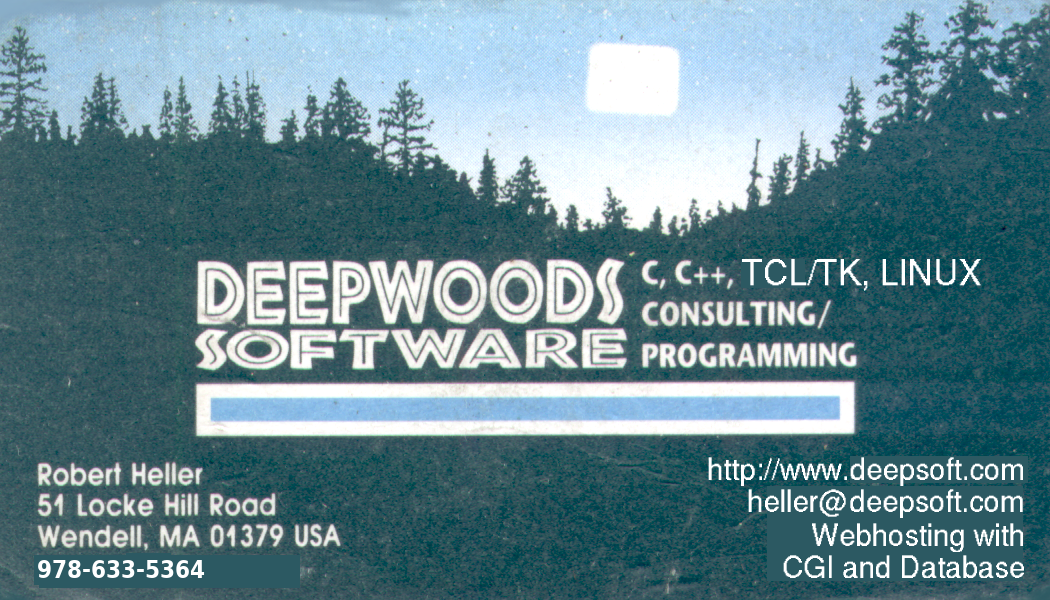
\includegraphics{NewCard.png}

\end{document}
